\chapter{Selector de programa a executar} \label{ch:selector}

\section{Objectius}

Durant el desenvolupament de les pràctiques, anem acumulant molts programes
petits i cridem el que volguem executar des de \fname{main}. Ens proposem
fer un \textbf{carregador} que pregunti a l'usuari quin dels programes
vol executar, i llavors li passi el control. D'aquesta forma, ja no haurem
d'estar modificant el \fname{main}, compilant i tornant a pujar si volem
fer servir un altre programa.

\section{Desenvolupament}

Començarem dissenyant l'interficie d'usuari. Proposem que el menú sigui una
vista lliscant de totes les opcions, on cadascuna es pinta en una fila
del display, i l'opció seleccionada tingui davant una fletxa. L'usuari pot
fer servir l'encoder per moure la selecció amunt o avall, i la 'vista'
(les opcions que es veuen a la pantalla) s'actualitza. Aquest és un sistema
molt comú en molts dispositius amb entrada limitada.

Per exemple, aquest seria l'estat inicial:
%
\begin{center}
  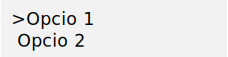
\includegraphics[width=11em]{../\projectname/initial-design}
\end{center}
%
I en girar l'encoder dues posicions tindriem:
%
\begin{center}
  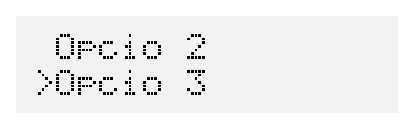
\includegraphics[width=11em]{../\projectname/initial-design-2}
\end{center}

En el moment que l'usuari vulgui executar el programa seleccionat, polsarà
el botó d'usuari.

Donat que el codi del selector només transferirà el control a la funció que
sigui, i que no hi ha gaire motiu perquè la resta del codi necessiti cridar
el selector o interactuar-hi, trobem oportú que estigui a \filename{main.c}
com un programa més, i que sigui aquest el que es cridi des del \fname{main}.

Ara farem una taula amb la informació de tots els programes que
tinguem fins ara. Cada programa serà un item d'aquesta taula: de moment l'item té
assignat un \emph{label} (text) i la funció que s'ha de cridar. Els noms han de ser curts,
ja que el nostre display només té 16 columnes i hem de deixar espai pels
elements de la interfície d'usuari.

\begin{minted}{c}
typedef struct {
    const char *text;
    void (*program)(void);
} MenuEntry;

MenuEntry menuEntries [] = {
    { "P1.8 LED Seq. ", ledSequence },
    { "P2.5 Backlight", backlightToggle },
    { "P2.6 LCD Init ", lcdJustInit },
    { "P2.7 LCD Hello", lcdHello },
    { "P2.7 LCD Names", putNamesOnDisplay },
    { "P3.4 Who_Am_I ", accelWhoAmI },
    { "P3.5 Accel Y  ", accelPollY },
    { "P3.6 Accel Dot", accelDrawAxis },
    { "P4.2 Interrupt", interruptTest },
    { "C1.2 Show key ", keyboardPoll },
    { "C1.2 Multi key", keyboardMultiPoll },
    { "C1.3 Intr. key", keyboardPollInterrupt },
    { "C2.4 Pot show ", potentiometerPoll },
    { "C2.5 Temp show", temperaturePoll },
    { "C2.6 Vdd show ", vddPoll },
    { "C3.3 Encoder  ", encoderPoll },
    { "R1.3 2Thd     ", test2threads },
    { "R1.3 2Thd +1  ", test2threadsPlus1 },
    { "R1.3 2Thd -1  ", test2threadsMinus1 },
    { "R1.3 2ThdSleep", test2threadsSleep },
    { "R1.3 4Thd     ", fourThreadsTest },
    { "R2.2 Sem      ", semaphoreExample },
    { "R2.2 Sem 2Thd ", semaphoreTwoThreads },
    { "R2.4 Mutex LCD", mutexExample },
};
#define MENU_ENTRIES_COUNT ((int32_t)(sizeof(menuEntries) / sizeof(MenuEntry)))
\end{minted}
\vskip -1em

Ara ja tenim aquesta informació organitzada i accessible de forma programàtica,
i si en el futur volem afegir una nova opció al menu, només hem d'afegir una entrada
a la taula. Les entrades es presentaran al menú amb el mateix ordre que figuren
aquí (cronològic), i s'ha inclòs davant de cada opció la pràctica i apartat on
es demanen.

La implementació de l'encoder en sí s'ha fet directament (\commit{9e907e7682a7c67f1085671d2e3aac4cf844b8fc}):

\begin{minted}{c}
void programSelector(void) {
    int32_t shift = 0, selection = 0, lastShift = -1, markerRow = -1;
    int32_t lastEncoder = encoderCount;

    // Initialize LCD
    LCD_Config(TRUE, FALSE, FALSE);

    while (1) {
        // Draw screen
        // -----------

        if (shift != lastShift) {
            // Redraw text labels
            int32_t row;
            for (row = 0; row < LCD_ROWS; row++) {
                LCD_GotoXY(1, row);
                LCD_SendString(menuEntries[shift + row].text);
            }
            lastShift = shift;
        }

        if (markerRow != selection - shift) {
            // Erase old selection marker
            if (markerRow != -1) {
                LCD_GotoXY(0, markerRow);
                LCD_SendChar(' ');
            }
            // Draw marker in new position
            markerRow = selection - shift;
            LCD_GotoXY(0, markerRow);
            LCD_SendChar('>');
        }

        // Sleep and update state
        // ----------------------

        SLEEP_MS(50);

        // If user button is pressed, execute selected program
        if ((BUTTON_PORT->IDR & BUTTON_BIT) != 0) {
            menuEntries[selection].program();
            while (1); // infinite loop, just in case the program returns
        }

        // Read encoder increment
        int32_t encoderIncrement = encoderCount - lastEncoder;
        lastEncoder += encoderIncrement;

        // Apply increment to selection, keeping it within valid bounds
        selection += encoderIncrement;
        if (selection < 0) selection = 0;
        if (selection >= MENU_ENTRIES_COUNT) selection = MENU_ENTRIES_COUNT - 1;

        // Scroll entries as needed to keep selection visible
        if (selection < shift) shift = selection;
        if (selection > (shift + LCD_ROWS - 1)) shift = selection - (LCD_ROWS - 1);
    }
}
\end{minted}
\vskip -1em

Es tracta d'un bucle infinit que fa les següents tasques:

\begin{enumerate}
\item Pintar el que calgui a la pantalla (si es tracta de la primera iteració ho pintarà tot)
\item Fer una petita espera
\item Si el botó d'usuari està premut, executar el programa seleccionat
\item Si l'encoder s'ha girat, actualitzar la selecció
\end{enumerate}

Observem que, quan s'executa el programa seleccionat, s'afegeix un bucle infinit després
perquè en cas que el programa retorni, la placa es quedi aturada. Reinicialitzar el selector
inmediatament seria complex i confús per l'usuari. En qualsevol cas, el selector no retorna mai.

Ara només queda cridar el selector des de \fname{main} un cop s'han fet totes
les inicialitzacions. La funció queda així (\commit{8e3868a06ffbebf662f902e4ef5fa24188df0eed}):

\begin{minted}{c}
int main(void) {
    // Basic initializations
    baseInit();
    LCD_Init();
    initAccel();
    initKeyboard();
    initEncoder();
    initADC();

    // Start selector
    programSelector();
    return 0;
}
\end{minted}
\vskip -1em

Al final es retorna zero perquè el compilador no doni problemes, però com ja s'ha comentat abans
el selector no hauria de retornar mai.

El programa es puja a la placa i es verifica el seu correcte funcionament, després d'arreglar dues errades.
El resultat es pot veure a la figura~\ref{fig:selector-board-initial} (estat inicial) i a
la figura~\ref{fig:selector-board-use} (després de fer un scroll).

\begin{figure}[p] %FIXME: subfigures?
  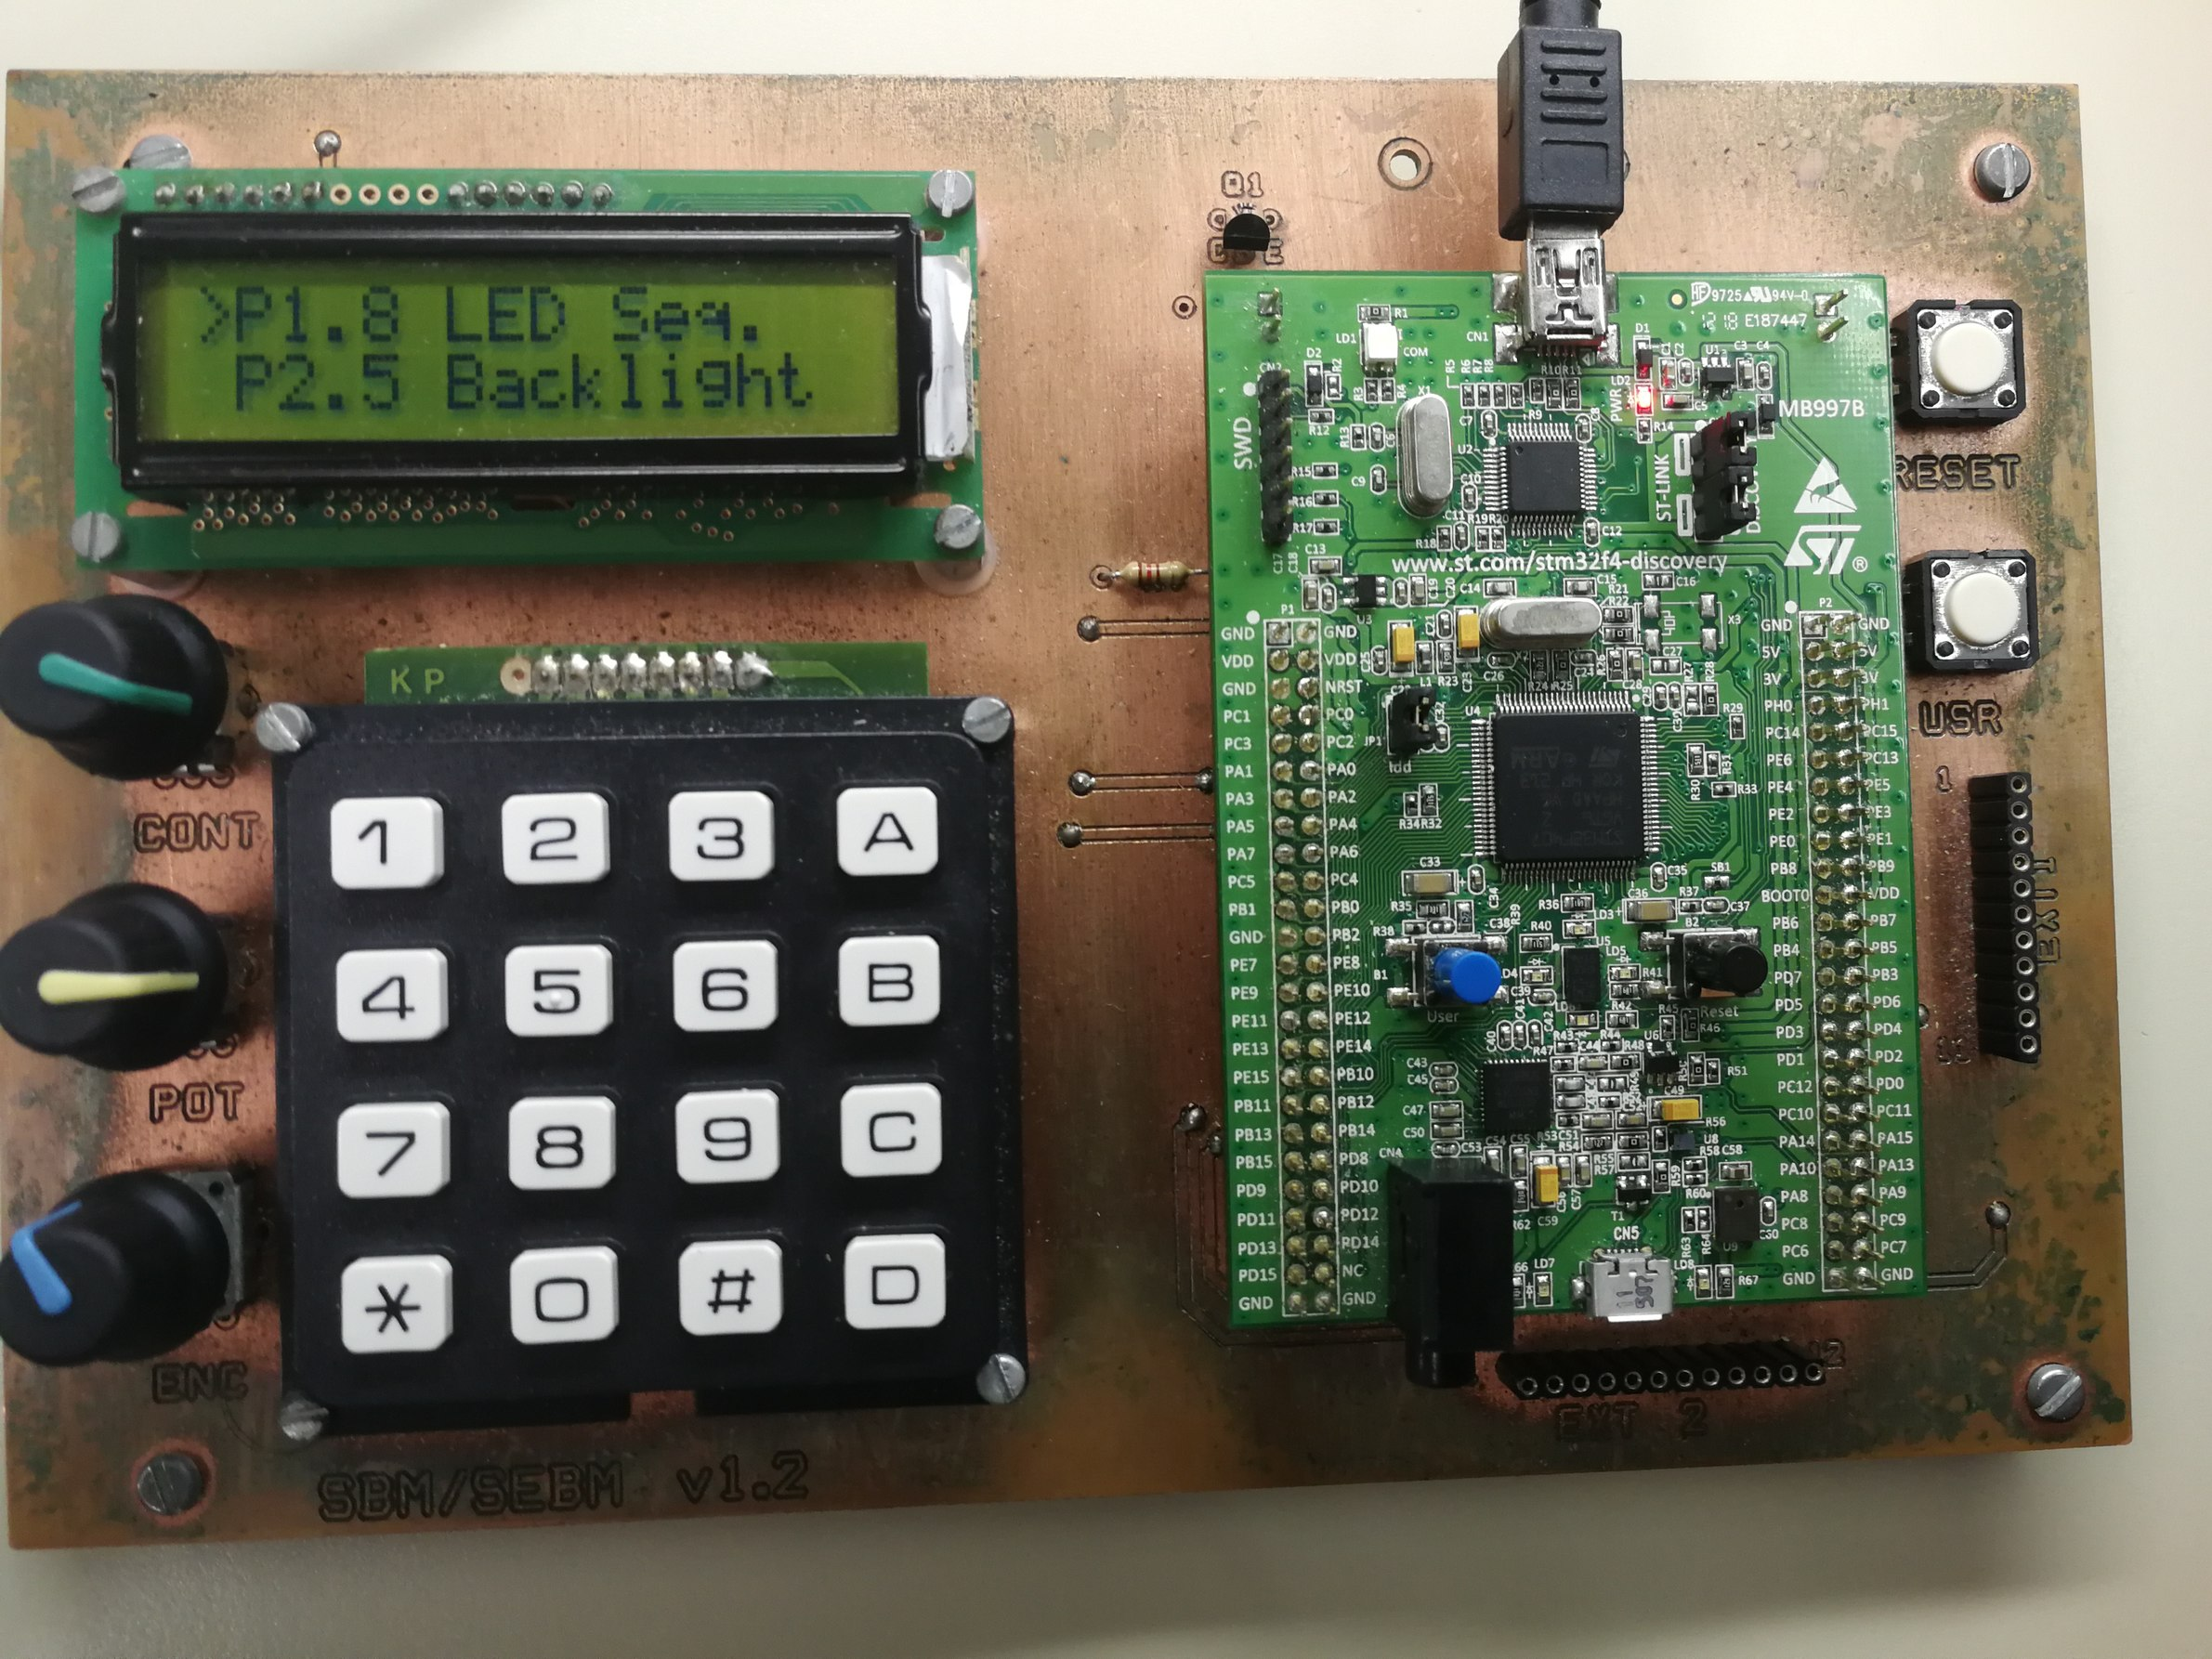
\includegraphics[width=.82\columnwidth]{../photos/board/selector-initial}
  \caption{ \label{fig:selector-board-initial} La placa executant el selector de programa, en l'estat inicial. }
\end{figure}
\begin{figure}[p]
  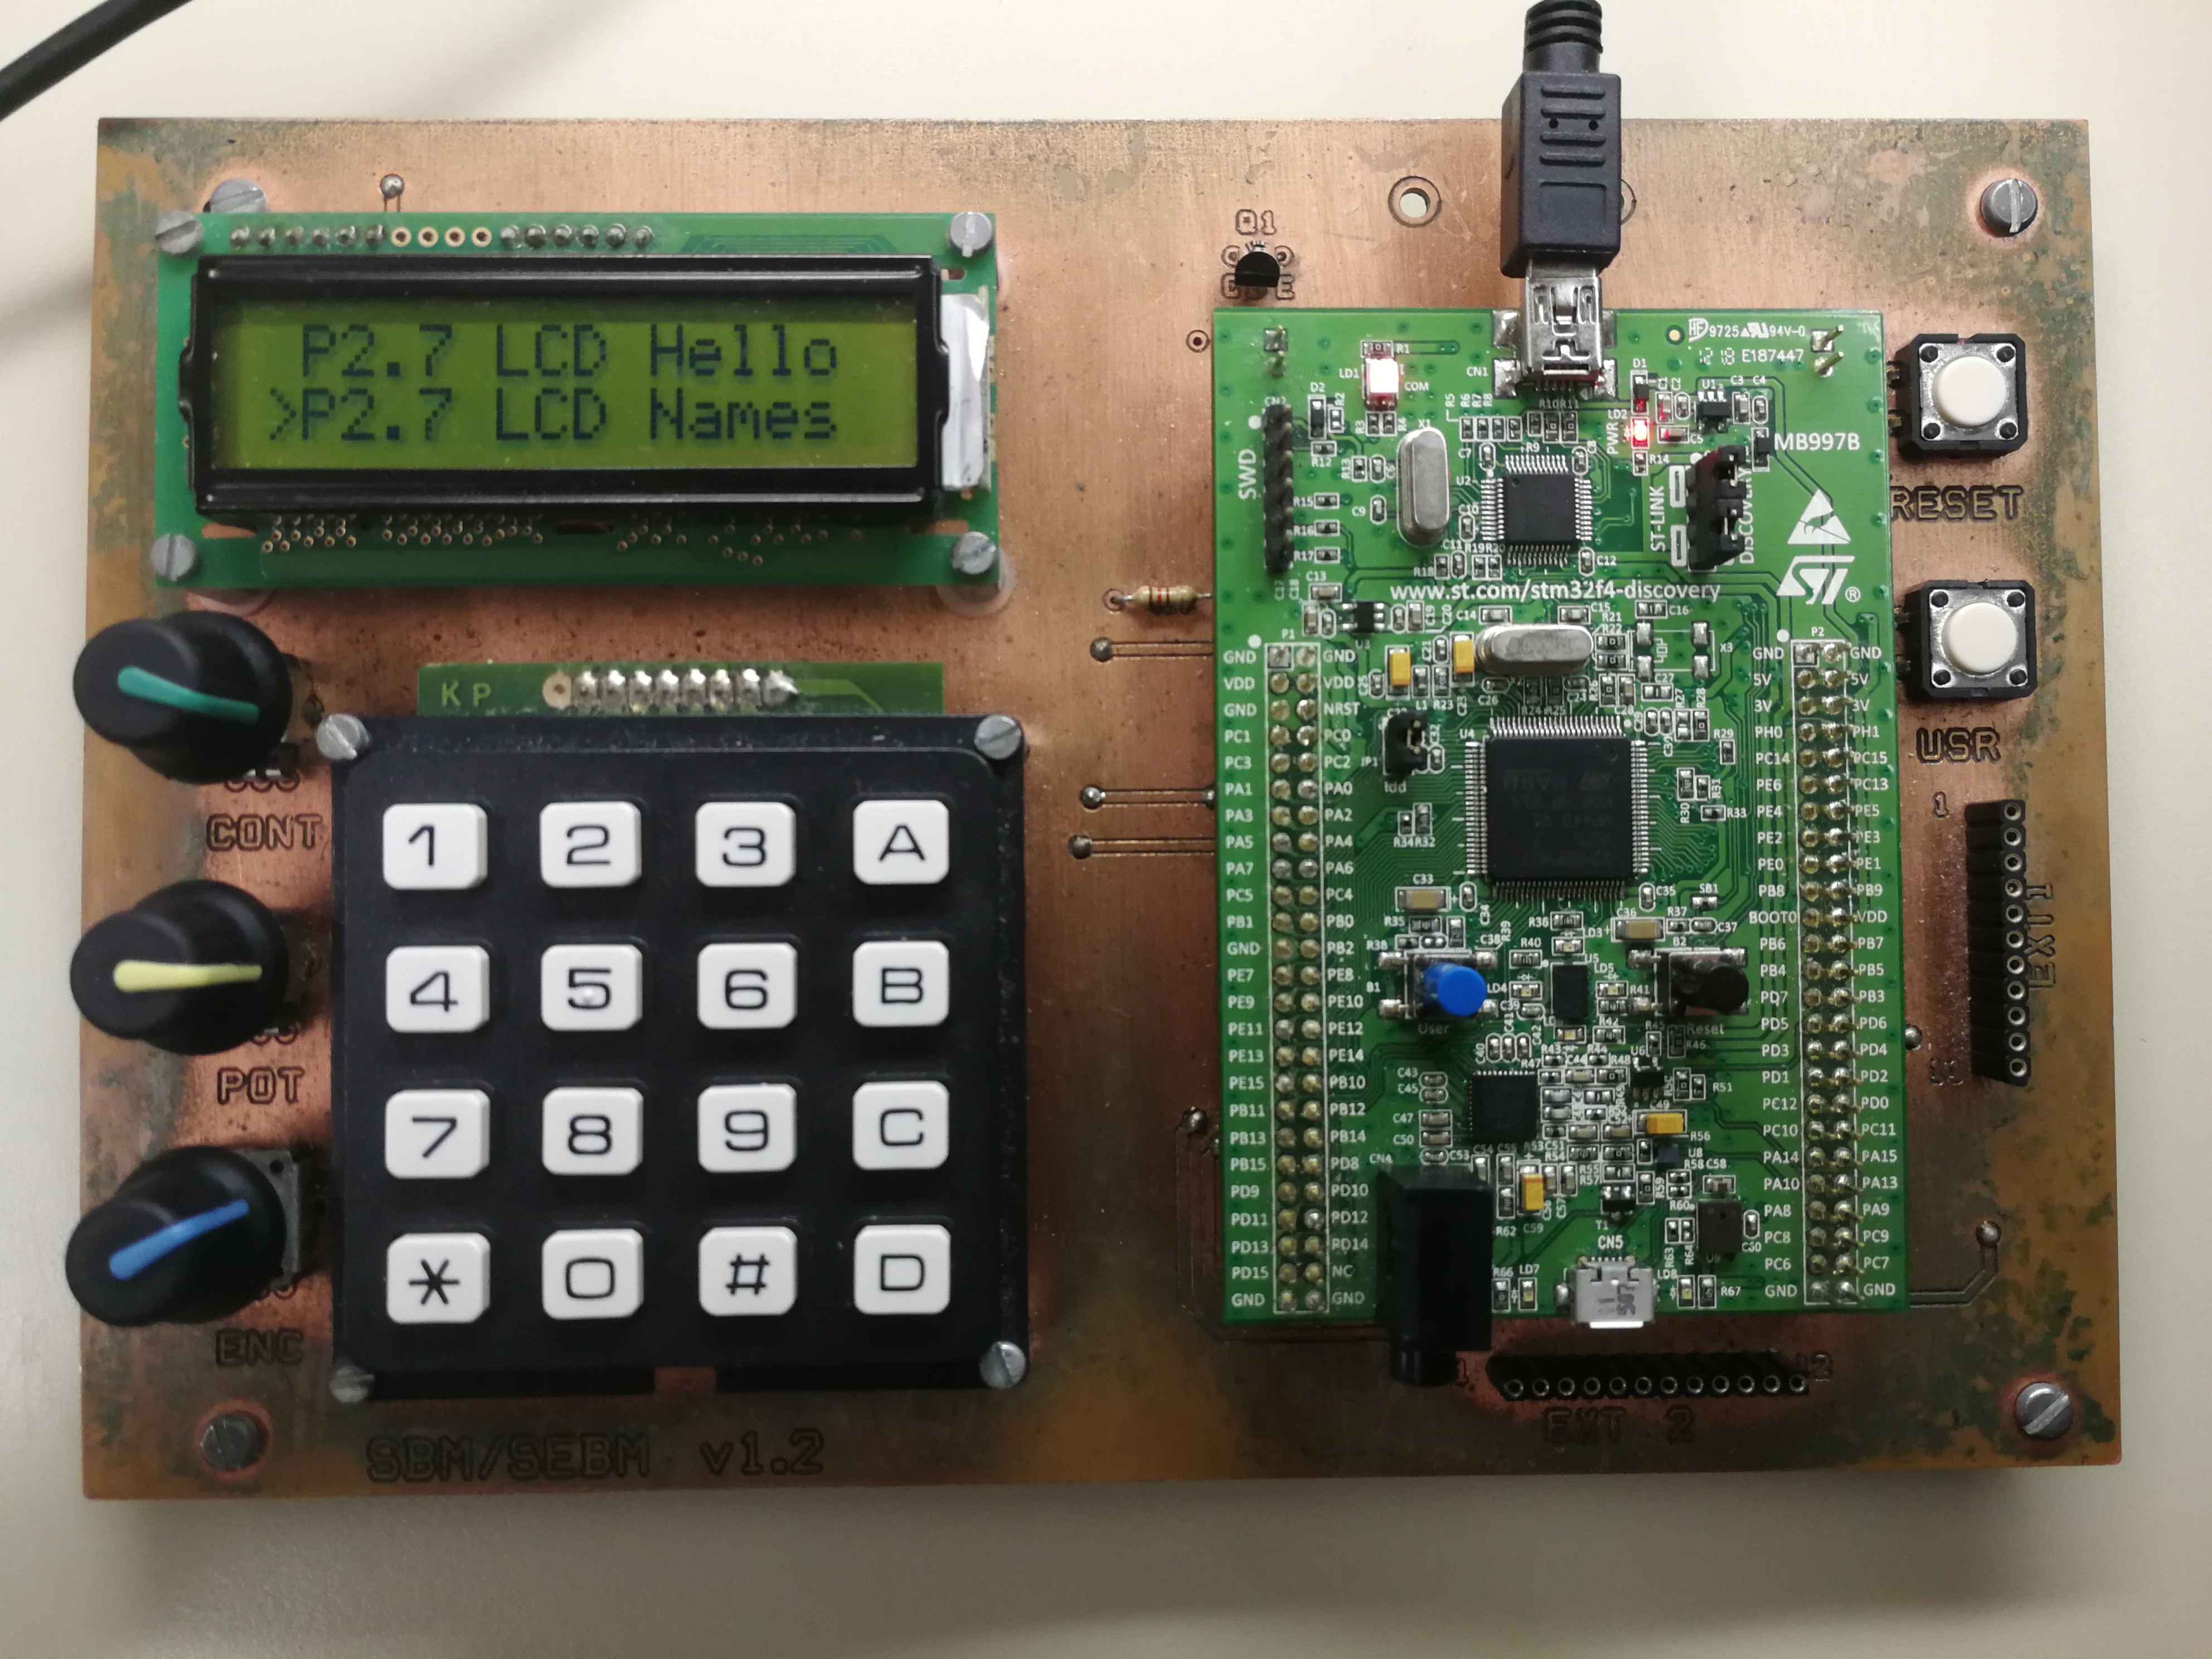
\includegraphics[width=.82\columnwidth]{../photos/board/selector-use}
  \caption{ \label{fig:selector-board-use} La placa executar el selector de programa, després de fer scroll. }
\end{figure}


\section{Conclusió}

Estic bastant contenta amb el resultat!

\section{Ajustaments posteriors}

Més endavant, com a part del \commit{241d2758d4a8a48d79a505b42816723ad34f37de} es neteja
la pantalla cridant \fname{LCD_ClearDisplay} abans de passar el control al programa.
Això es fa per evitar confusió i
deixar clar que el selector ja no s'executa, per a programes senzills que no toquen l'LCD.

També, el \commit{cb2027c662950e206d1340a2cab5bdee77aa0a4a} arregla un petit bug del selector
(no s'estava netejant la pantalla en iniciar-se) i afegeix un caràcter d'espai entre la fletxa i
la descripció de l'item, fent que ara aquesta comenci en la tercera columna:

\begin{minted}{diff}
--- a/main.c
+++ b/main.c
@@ -510,6 +510,7 @@ void programSelector(void) {
     int32_t lastEncoder = encoderCount;
 
     // Initialize LCD
+    LCD_ClearDisplay();
     LCD_Config(TRUE, FALSE, FALSE);
 
     while (1) {
@@ -520,7 +521,7 @@ void programSelector(void) {
             // Redraw text labels
             int32_t row;
             for (row = 0; row < LCD_ROWS; row++) {
-                LCD_GotoXY(1, row);
+                LCD_GotoXY(2, row);
                 LCD_SendString(menuEntries[shift + row].text);
             }
             lastShift = shift;
\end{minted}
\vskip -1em

